\documentclass[main.tex]{subfiles}

\begin{document}

\begin{q}{5}
Consider an observer at the equator and a star at $A = \ang{70}$ and $h =
\ang{0}$. Calculate the star's $A$ and $h$ after $1$ hour.

\noindent\textit{Hint: Assume that after $1$ hour, the star is at point $A$.
Draw a great circle passing through the zenith and point $A$. Let $B$ be the
point where the great circle intersects the horizon. Let the north celestial
pole be point $C$. Consider the spherical triangle $ABC$. Assume that the radius
of the celestial sphere is $1$ unit. Hence,the lengths of side $c$ and side $a$
correspond to the altitude and azimuth of the star, respectively.}
\begin{enumerate}[label=\text{(\alph*)}]
    \item What is the angle $B$?
    \item What is the angle $C$?
    \item What is the length of side $b$?
    \item By using a law of spherical trigonometry, calculate the length of side
    $c$.
    \item By using a law of spherical trigonometry, calculate the length of side
    $a$.
\end{enumerate}
\end{q}

\begin{sol}
Consider the following celestial sphere construction with spherical triangle
$ABC$ bound by $A$ (position of star $\SI{1}{\hour}$ later), $B$, $C$ (NCP):
\begin{figure}[h!]
    \centering
    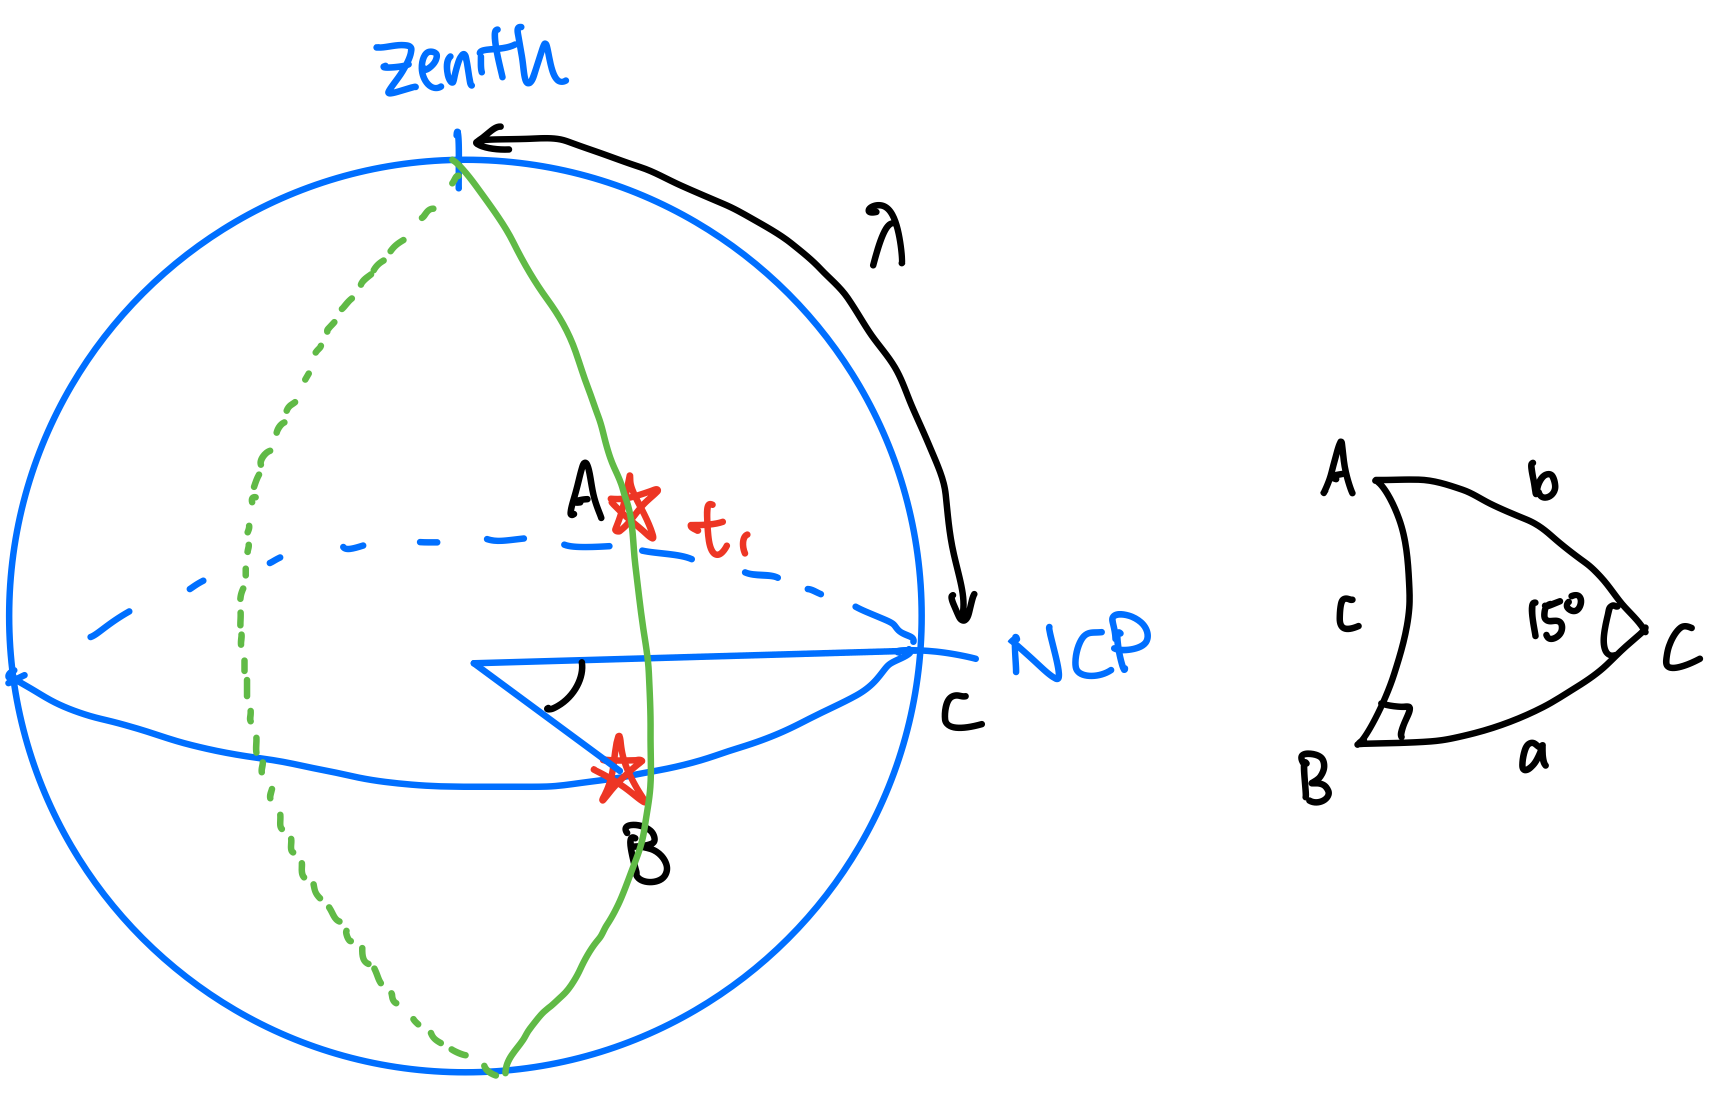
\includegraphics[width=0.5\textwidth]{figure2}
\end{figure}

\begin{subsol}
Since the great circle containing arc $AB$ passes through the zenith, a pole of
the horizon plane of the observer, $B = \ang{90}$.
\end{subsol}

\begin{subsol}
Since the observer is at the equator, the point $\paren{A = \ang{0},~h =
\ang{0}}$ coincides with the north celestial pole, $C = \ang{90}$, $C$ is equal
in value to the change in hour angle of the star. Hence,
\begin{equation}
    C = \ra{-5} - \paren{\ra{-6}} = \ang{15}.
\end{equation}  
\end{subsol}

\begin{subsol}
Similarly, when the star is at $\paren{A = \ang{70},~h = \ang{0}}$, the star has
a declination angle,
\begin{equation}
    \delta = \ang{90} - \ang{70} = \ang{20}.
\end{equation}
Thus, since $b$ is the angular distance between the position of the star 1 hour
later and the NCP,
\begin{equation}
    b = \ang{90} - \delta = \ang{90} - \ang{20} = \ang{70}.
\end{equation} 
\end{subsol}

\newpage
\begin{subsol}
By the law of sines for spherical triangles,
\begin{equation}
    \frac{\sin c}{\sin C} = \frac{\sin b}{\sin B}
\end{equation}
\begin{equation}
    \begin{split}
        \implies\quad c &= \arcsin{\paren{\frac{\sin b\sin C}{\sin B}}} = \arcsin\paren{\frac{\sin\ang{70}\sin\ang{15}}{\sin\ang{90}}} = \ang{14.08}\\
        &\approx \ang{14}
    \end{split}.
\end{equation} 
\end{subsol}

\begin{subsol}
By the cotangent four-part formula,
\begin{equation}
    \cos\text{IS}\cos\text{IA} = \cot\text{OS}\sin\text{IS} - \cot\text{OA}\sin\text{IA},
\end{equation}
which applied to spherical triangle $ABC$, gives,
\begin{equation}
    \cos a\cos C = \cot b\sin a - \cot B \sin C
\end{equation}
\begin{equation}
    \begin{split}
        \implies\quad a &= \arctan\paren{\frac{\cos C}{\cot b}} = \arctan{\paren{\frac{\cos\ang{15}}{\cot\ang{70}}}} \approx \ang{69.35}\\
        &\approx \ang{69}.
    \end{split}
\end{equation}
\end{subsol}

\end{sol}

\end{document}
